\documentclass[a4paper,12pt]{report}

\usepackage[utf8]{inputenc}
\usepackage[T1]{fontenc}
\usepackage{xcolor,graphicx}
\usepackage[top=0.6in,bottom=0.6in,right=1in,left=1in]{geometry}

\definecolor{blue}{RGB}{31,56,100}

% Define parameters
\newcommand{\labnumber}{1}
\newcommand{\labtopic}{LAN CABLING}
\newcommand{\subjectname}{Computer Networks and Security}

\newcommand{\studentname}{Nimesh Poudel}
\newcommand{\studentid}{KAT078BCT054}
\newcommand{\studentgroup}{B1}
\newcommand{\studentyear}{IV/I}

\begin{document}

% titlepage.tex

\begin{titlepage}
\begin{center}

% Header section
\begin{minipage}{2.5cm}
	\begin{center}
		
\includegraphics[height=2.5cm]{./logo/kec.png}
	\end{center}
\end{minipage}\hfill
\begin{minipage}{10cm}
	\begin{center}
	\Large{\textbf{KATHMANDU ENGINEERING COLLEGE}}\\[0.1cm]
    \small{KALIMATI, KATHMANDU}\\[0.1cm]
    \textbf{TRIBHUVAN UNIVERSITY}
	\end{center}
\end{minipage}\hfill
\begin{minipage}{2.5cm}
	\begin{center}
		
\includegraphics[height=2.5cm]{./logo/tu.jpg}
	\end{center}
\end{minipage}

\vspace{3.5cm}

{\huge \bfseries \uppercase{lab report on} \\[0.5cm] }
{\large \bfseries \subjectname}

\vspace{2.5cm}
{\large \bfseries LAB NO: \labnumber}\\[0.5cm]

\rule{\linewidth}{0.3mm} \\[0.4cm]
{ \huge \bfseries\color{black} \labtopic \\[0.4cm] }
\rule{\linewidth}{0.3mm} \\[3cm]

% Author and supervisor
\begin{tabular}{c @{\hspace{4cm}} c}
    \Large{\textbf{Submitted by:}} & \Large{\textbf{Submitted to:}} \\[1em]
   \large{\MakeUppercase{\studentname}} & \uppercase{Department} \\[0.5em]
    \large{\texttt{\studentid}} & \uppercase{of} \\[0.5em]
    \MakeUppercase{Group: \studentgroup} & \uppercase{Computer} \\[0.5em]
    \MakeUppercase{Year: \studentyear}& \uppercase{Engineering}
\end{tabular}

\vfill

\textbf{\today}

\end{center}
\end{titlepage}



\chapter*{\centering \labtopic}
\section*{Required Components}
\begin{itemize}
    \item LAN Cable
    \item Crimping Tool
    \item RJ45
    \item Tester
\end{itemize}

\section*{Theory}
\subsection*{LAN Cable}
A LAN (Local Area Network) cable is a type of cable used to connect computers, printers, routers, and other devices in a small area like home, offices, schools, etc. It helps to transfer data quickly between these devices so that they can share files, the Internet, and other resources. The most common type of LAN cable is the Ethernet cable, which usually has an RJ45 connector at both ends. These cables are easy to use and provide a stable and fast connection, making them important for building a reliable network.\\
\begin{figure}[h]
    \centering
    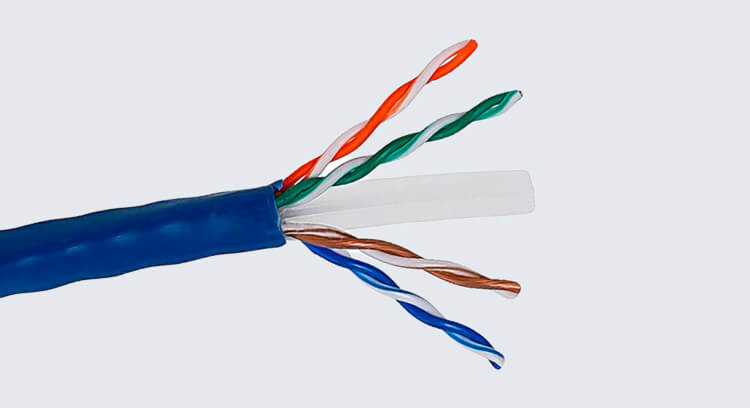
\includegraphics[width=0.9\linewidth]{lan-cable.jpg}
    \caption{LAN Cable}
    \label{fig:lan_cable}
\end{figure}

\subsection*{Cabling Standard}
Cabling standards are the rules that explain how network cables should be connected and arranged. These standards help make sure that the cables work properly and can be used in different devices around the world. By following these standards, we can avoid connection problems and ensure good communication between devices in a network. One of the most common cabling standards used in networking is the TIA/EIA-568 standard.
\subsubsection*{568A Standard}
The 568A standrad is one of the two main standards used for Ethernet cables. It is commonly used in residential networks and preferred by some government projects. In this green colored cables are placed before orange one. The order from pin one to pin eight is:


\begin{enumerate}
    \item Green White
    \item Green
    \item Orange White
    \item Blue
    \item Blue White
    \item Orange
    \item Brown White
    \item Brown
\end{enumerate}

This specific order helps to ensure proper signal transmission and is followed when creating straight-through or crossover cables.

\subsubsection*{568B Standard}
The 568B wiring standard is more commonly used in commercial and older installations. It switches the position of the green and orange wire pairs to 568A. In this standarad orange wire comes first. The color order from pin one to pin eight is:

\begin{enumerate}
    \item Orange White
    \item Orange
    \item Green White
    \item Blue
    \item Blue White
    \item Green
    \item Brown White
    \item Brown
\end{enumerate}

568B is widely used because it became poplular standarad over time, especially in offices A and large network setups. Like 568A, it ensures the correct flow of data across network and devices. 
\newpage
\subsection*{Straight Cable}
A straight cable is a type of Ethernet cable where both ends have the same wiring standard. either 568A to 568A or 568B to 568B. This means the wire colors are arranged in the same order on both connectors. Straight cables are used to connect different types of devices, such as a computer to a switch, a router to a switch, or a PC to a hub, These cables are very common and are usually used in most home and office networks. For example, if you are connecting your computer to your internet router, you will likely use a straight cable.
\begin{figure}[h]
    \centering
    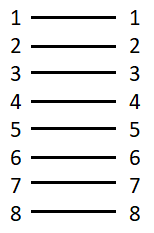
\includegraphics[width=0.2\linewidth]{straight-cable.png}
    \caption{Straight cable pin connection}
\end{figure}
\subsection*{Crossover Cable}
A crossover cable is an Ethernet cable where one end follows the 568A standard and the other end follows the 568B standard. This means the wire colors are arranged differently on each side. Crossover cables are used to connect similar types of devices, such as PC to PC, switch to switch, router to router, or hub to hub. There are also some exceptions where devices that look different are treated as similar. For example, PC to router and switch to hub are considered similar devices and need a crossover cable in older network setups. These connections require the transmit and receive signals to cross over. However, most modern devices support Auto-MDI/MDIX, which allows them to automatically adjust and work with either a straight or crossover cable. Still, it's important to know the correct cable ty-especially for labs and manual configurations.
\begin{figure}[h]
    \centering
    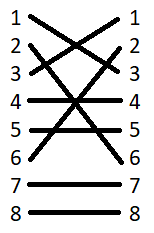
\includegraphics[width=0.2\linewidth]{crossover_cable.png}
    \caption{Crossover cable pin connection}
\end{figure}
\newpage
\subsection*{Cable Category Table}
There are different types of LAN cables, called categories, which are designed to support different speeds and applications. The table below shows the common LAN cable categories from Category 3 to the latest Category 8, including their maximum data speeds, and typical uses: 
\begin{table}[h]
\centering
\begin{tabular}{|c|c|c|}
    \hline
     Category & Maximum Data Speed & Applications\\ \hline
     Cat3 & 10 Mbps & Old telephone lines, 10BASE-T Ethernet \\
     Cat4 & 16 Mbps & Token Ring Networks (rare/obsolete) \\
     Cat5 & 100 Mbps & Early Ethernet, 100BASE-TX \\
     Cat5e & 1 Gbps & Gigabit Ethernet, 1000BASE-T \\
     Cat6 & 1 Gbps (Upto 55m) & Fast network, used in office \\
     Cat6a & 10 Gbps & High speed network, Data center \\
     Cat7 & 10 Gbps & Shielded Networks, Server Rooms \\
     Cat8 & 25-40 Gbps & Data center, High speed server \\ \hline
\end{tabular}
\caption{LAN Cabel category, Speed and applications}
\end{table}
\section*{Procedure}
\begin{enumerate}
    \item Take a Cat6 LAN cable and use a crimping tool to carefully remove the outer jacket of the cable.
    \item Untwist the twisted pairs of wires inside and straighten each wire individually.
    \item Remove the plastic cross skeleton (present in Cat6 cables) to make handling easier.
    \item Arrange the wires according to the selected standard standard (on both ends) or crossover cable (different standards on each end), following the 568A or 568B wiring schemes.
    \item Trim the wires to make them equal in length for a clean fit into the connector. that all wires stay in the
    \item Insert the wires carefully into the RJ45 connector, ensuring correct order and reach the end of the connector.
    \item Use the crimping tool to securely clamp the RJ45 connector, locking the wires in place.
    \item Repeat the same process for the other end of the cable.
    \item Use a cable tester to check the connectivity and confirm that the cabling is done correctly.
\end{enumerate}
\section*{Result}
A Cat6 crossover Ethernet cable was successfully created using 568A and 568B standard. After crimping and assembling the cable, a LAN cable tester was used to verify the connection. The tester showed that all the pins were correctly connected in the same order on both sides (1 to 3, 2 to 6, 3 to 1, 4 to 4, 5 to 5, 6 to 2, 7 to 7, 8 to 8), confirming that the cable was working properly and suitable for network communication between different devices.
\section*{Discussion}
LAN cabling is a fundamental part of networking that ensures reliable communication between devices. In this lab, different aspects of LAN cable creation were explored, including cable types (straight and crossover), wiring standards (568A and 568B), and proper use of tools like crimping tools and cable testers. Understanding the difference between straight and crossover cables is essential, as each serves a specific purpose depending on the devices being connected. Proper cable preparation, such as stripping the outer jacket, untwisting and arranging the wire pairs, and securing them in RJ45 connectors, is crucial for ensuring a functional and durable connection. Testing the cable confirms the accuracy of the wiring and the effectiveness of the crimping process. This practical exercise helps reinforce theoretical knowledge about physical network setup and troubleshooting.
\section*{Conclusion}
The LAN cabling lab provided hands-on experience in preparing and assembling Ethernet cables using the correct standards and procedures. It highlighted the importance of understanding cable types, wiring schemes, and the correct use of tools in networking. By the end of the lab, the creation and testing of both straight and crossover cables reinforced the essential skills needed for building and maintaining a functional local area network. This foundational knowledge is critical for anyone involved in network installation or support.
\end{document}